\subsection{Zero absoluto: Determinação do zero absoluto utilizando um termômetro a
gás}

Conforme a descrição na metodologia, os primeiros dados coletados neste experimento foram os relativos às pressões do gás do sistema para determinadas temperaturas descritas nas quatro condições a seguir:

\begin{enumerate}
    \item Bulbo mergulhado em água à temperatura ambiente;
    \item Bulbo mergulhado em gelo em fusão;
    \item Bulbo mergulhado em nitrogênio líquido;
    \item Bulbo mergulhado em água em ebulição.
\end{enumerate}

Lembrando que as pressões são determinadas diretamente pela leitura da altura h da coluna no experimento, sendo que h é obtido pela diferença das alturas em dois pontos distintos do termômetro em “U”. Dessa forma, temos a seguinte tabela com os dados, numerados de acordo com cada condição:

\begin{table}[H]
    \centering
    \begin{tabular}{ |c||c||c| }
        \hline
        \textbf{Condição} & \textbf{Temperatura (ºC)} & \textbf{Pressão (cmHg)}\\
        \hline 
        1       & 24,7     & $h = 81 - 12 = 69$  \\
        2       & 1,0      & $h = 78 - 15 = 63$  \\
        3       & -196,0   & $h = 55,4 - 37,5 = 17,9$ \\
        4       & 97,0     & $h = 87,8 - 5,5 = 82,3$ \\
        \hline
        \end{tabular}
    \caption{Valores de Temperatura e Pressão para cada condição estabelecida no experimento conforme a enumeração.} 
\end{table}

Após isso, construímos um gráfico da pressão (medida em cmHg) em função da temperatura (medida em ºC), que pode ser visualizado na imagem abaixo:

\begin{figure}[H]
  \centering
  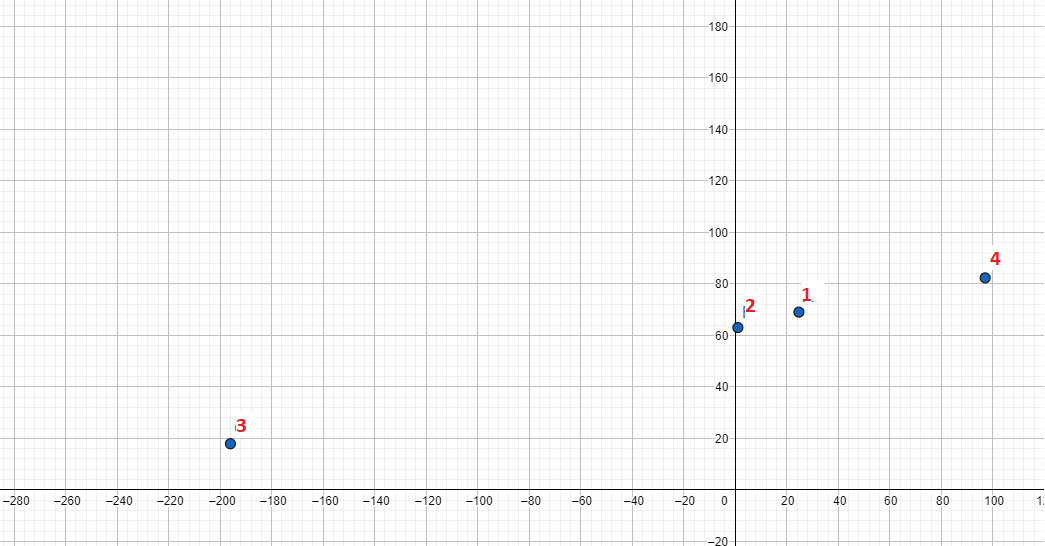
\includegraphics[scale=0.5]{images/Gráfico 1 - experimento 3.png}
  \caption{Gráfico da Pressão (cmHg) em função da Temperatura (ºC).}
\end{figure}

Utilizando o aplicativo “Least Squares” para Android, determinamos o coeficiente de dilatação do gases ideais a volume constante ($\beta$) e o valor de $P_0$ a partir do método dos mínimos quadrados. O resultado da aplicação desse método pode ser visualizado na imagem a seguir:

\begin{figure}[H]
  \centering
  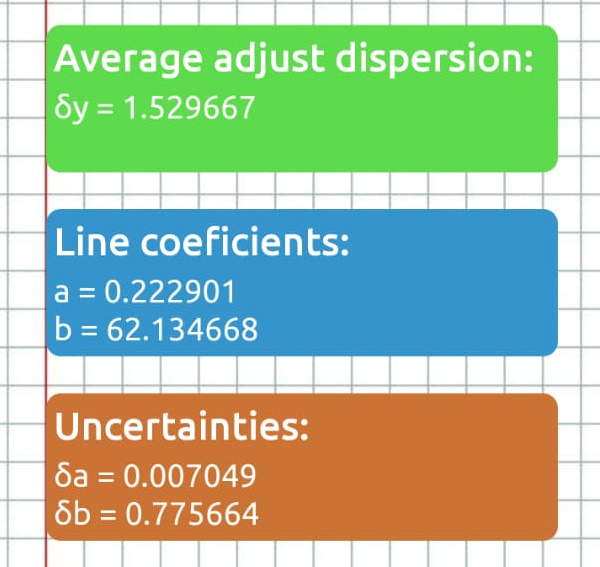
\includegraphics[scale=0.6]{images/Gráfico 2 - experimento 3.png}
  \caption{Aplicação do Método dos Mínimos Quadrados para encontrar os valores do coeficiente angular (a) e do coeficiente linear (b).}
\end{figure}

Na análise gráfica, determinamos, então, o coeficiente de dilatação dos gases ideais a volume constante $\beta$ e o valor de $P_0$:

\[ b (\textbf{coeficiente linear}) = P_0 = 62,1 cmHg\]\
\[ a (\textbf{coeficiente angular}) = P_0 \cdot \beta \longrightarrow \beta = \frac{0,222901}{62,1} = 0,003589\]\

Portanto, sabendo os valores de $\beta$ e $P_0$, podemos escrever a equação que descreve esse comportamento do gráfico da pressão (medida em cmHg) em função da temperatura (medida em ºC), sendo igual a:

\[ P(T) = P_0 \cdot \beta \cdot T + P_0 \]\
\[ P(T) = 62,1 \cdot 0,003589 \cdot T + 62,1 \]\
\[ \therefore P(T) = 0,222901 \cdot T + 62,1 \]\

Após a determinação da equação acima, traçamos uma reta sobre os pontos experimentais e determinamos, com a extrapolação dessa reta, o zero absoluto:

\begin{figure}[H]
  \centering
  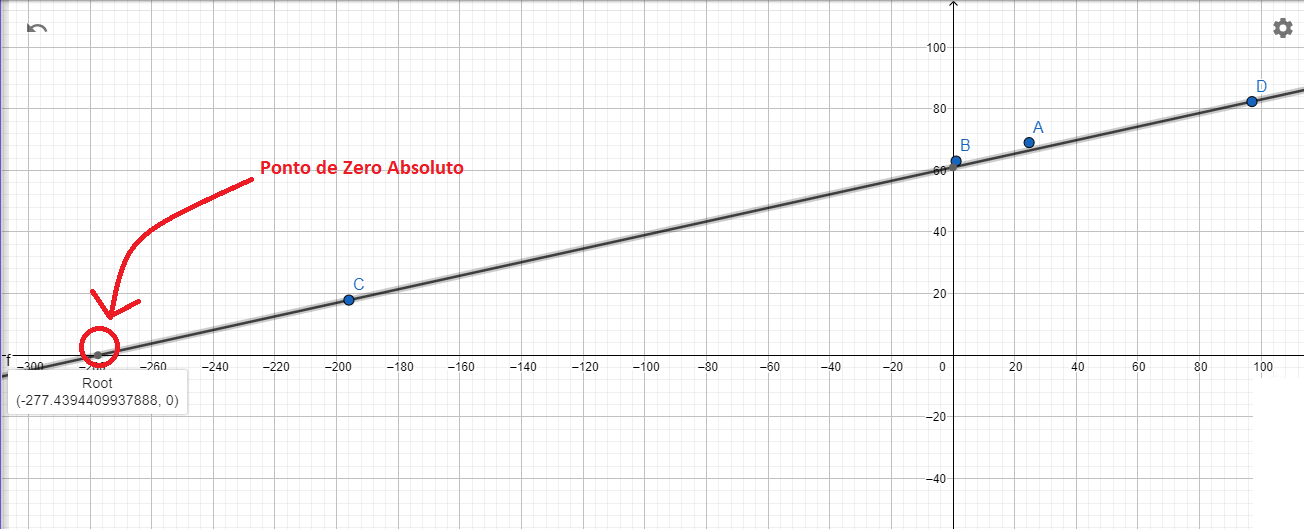
\includegraphics[scale=0.45]{images/Gráfico 3 - experimento 3.png}
  \caption{Equação da reta que define a pressão do gás em função da temperatura com sua respectiva extrapolação para determinação do zero absoluto.}
\end{figure}

Dessa forma, após uma análise gráfica, podemos determinar o valor correspondente do ponto de zero absoluto a partir de cálculos diretamente da equação que define a reta, lembrando que no zero absoluto a pressão do gás é dita conceitualmente igual a 0: 

\[ P(T) = P_0 \cdot \beta \cdot T + P_0 \]\
\[ 0 = 0,222901 \cdot T + 62,1 \]\
\[ -62,1 = 0,222901 \cdot T  \]\
\[ \frac{-62,1}{0,222901}  =  T  \]\
\[ \therefore \mathbf{T = -278,60 ^\circ C} \]\

Dessa forma, podemos concluir que o valor correspondente do ponto de zero absoluto é igual a $T_{Zero-Absoluto}= -278,60 ºC$. Conforme a literatura científica, a temperatura de zero absoluto é de aproximadamente $T_{Zero-Absoluto-Ref}= -273 ºC$, ou seja, podemos concluir que o valor alcançado experimentalmente é \textbf{satisfatório} dado que é muito próximo do valor de referência.
